%************************************************
\chapter{Task Allocation and Optimization}\label{ch:TA} % $\mathbb{ZNR}$
%************************************************
 Solving the \ac{TA} problem in this context means assigning weed detections to removal tools in the most efficient way. The idea is to find the best allocation of resources and the optimal sequence of stops, that will maximize the number of plants removed, and minimize the tools' idle time. The solution has to consider the constraints of the problem such as:

\begin{description}
    \item[Geometric Constraints:] A stop is considered valid only if the weeds lie within the workspaces of the tools (observe \autoref{fig:problem-layout.png}).
    \item[Movement Constraints:] The robot can only move forward in a straight line at a max speed of $0.3\frac{m}{s}$. % acceleration and deceleration times have to be considered.
    \item[Task Processing:] Each plant removal takes approximately $45$ seconds, during which the robot must remain stationary to ensure a successful extraction. Movement during this process is not allowed as it could compromise the tool operation.
    \item[Dynamic Environment:] Weed positions are initially unknown and are discovered dynamically during operation by the camera in front of the vehicle.
    \item[Processing Time:] The solution must run online because the robot discovers new weeds during operation, and decisions about stopping and \ac{TA} must adapt in real-time.
\end{description}

We define a '\textit{good}' stop as the next robot position that maximizes plant coverage while keeps a balance on the number of tasks assigned to each implement (aiming to minimize idle time). The problem can be approached in two ways: one option is to first determine the optimal stop location, after which task allocation becomes trivial by simply assigning tasks based on whether they fall within the front or back workspace. Alternatively, we can first allocate tasks to the implements and then compute the stop position that satisfies the corresponding geometric constraints. Both approaches are similar, differing mainly in the order of operations, but each perspective opens the door to different methods and algorithms to try.

\begin{figure}[bth]
    \centering
    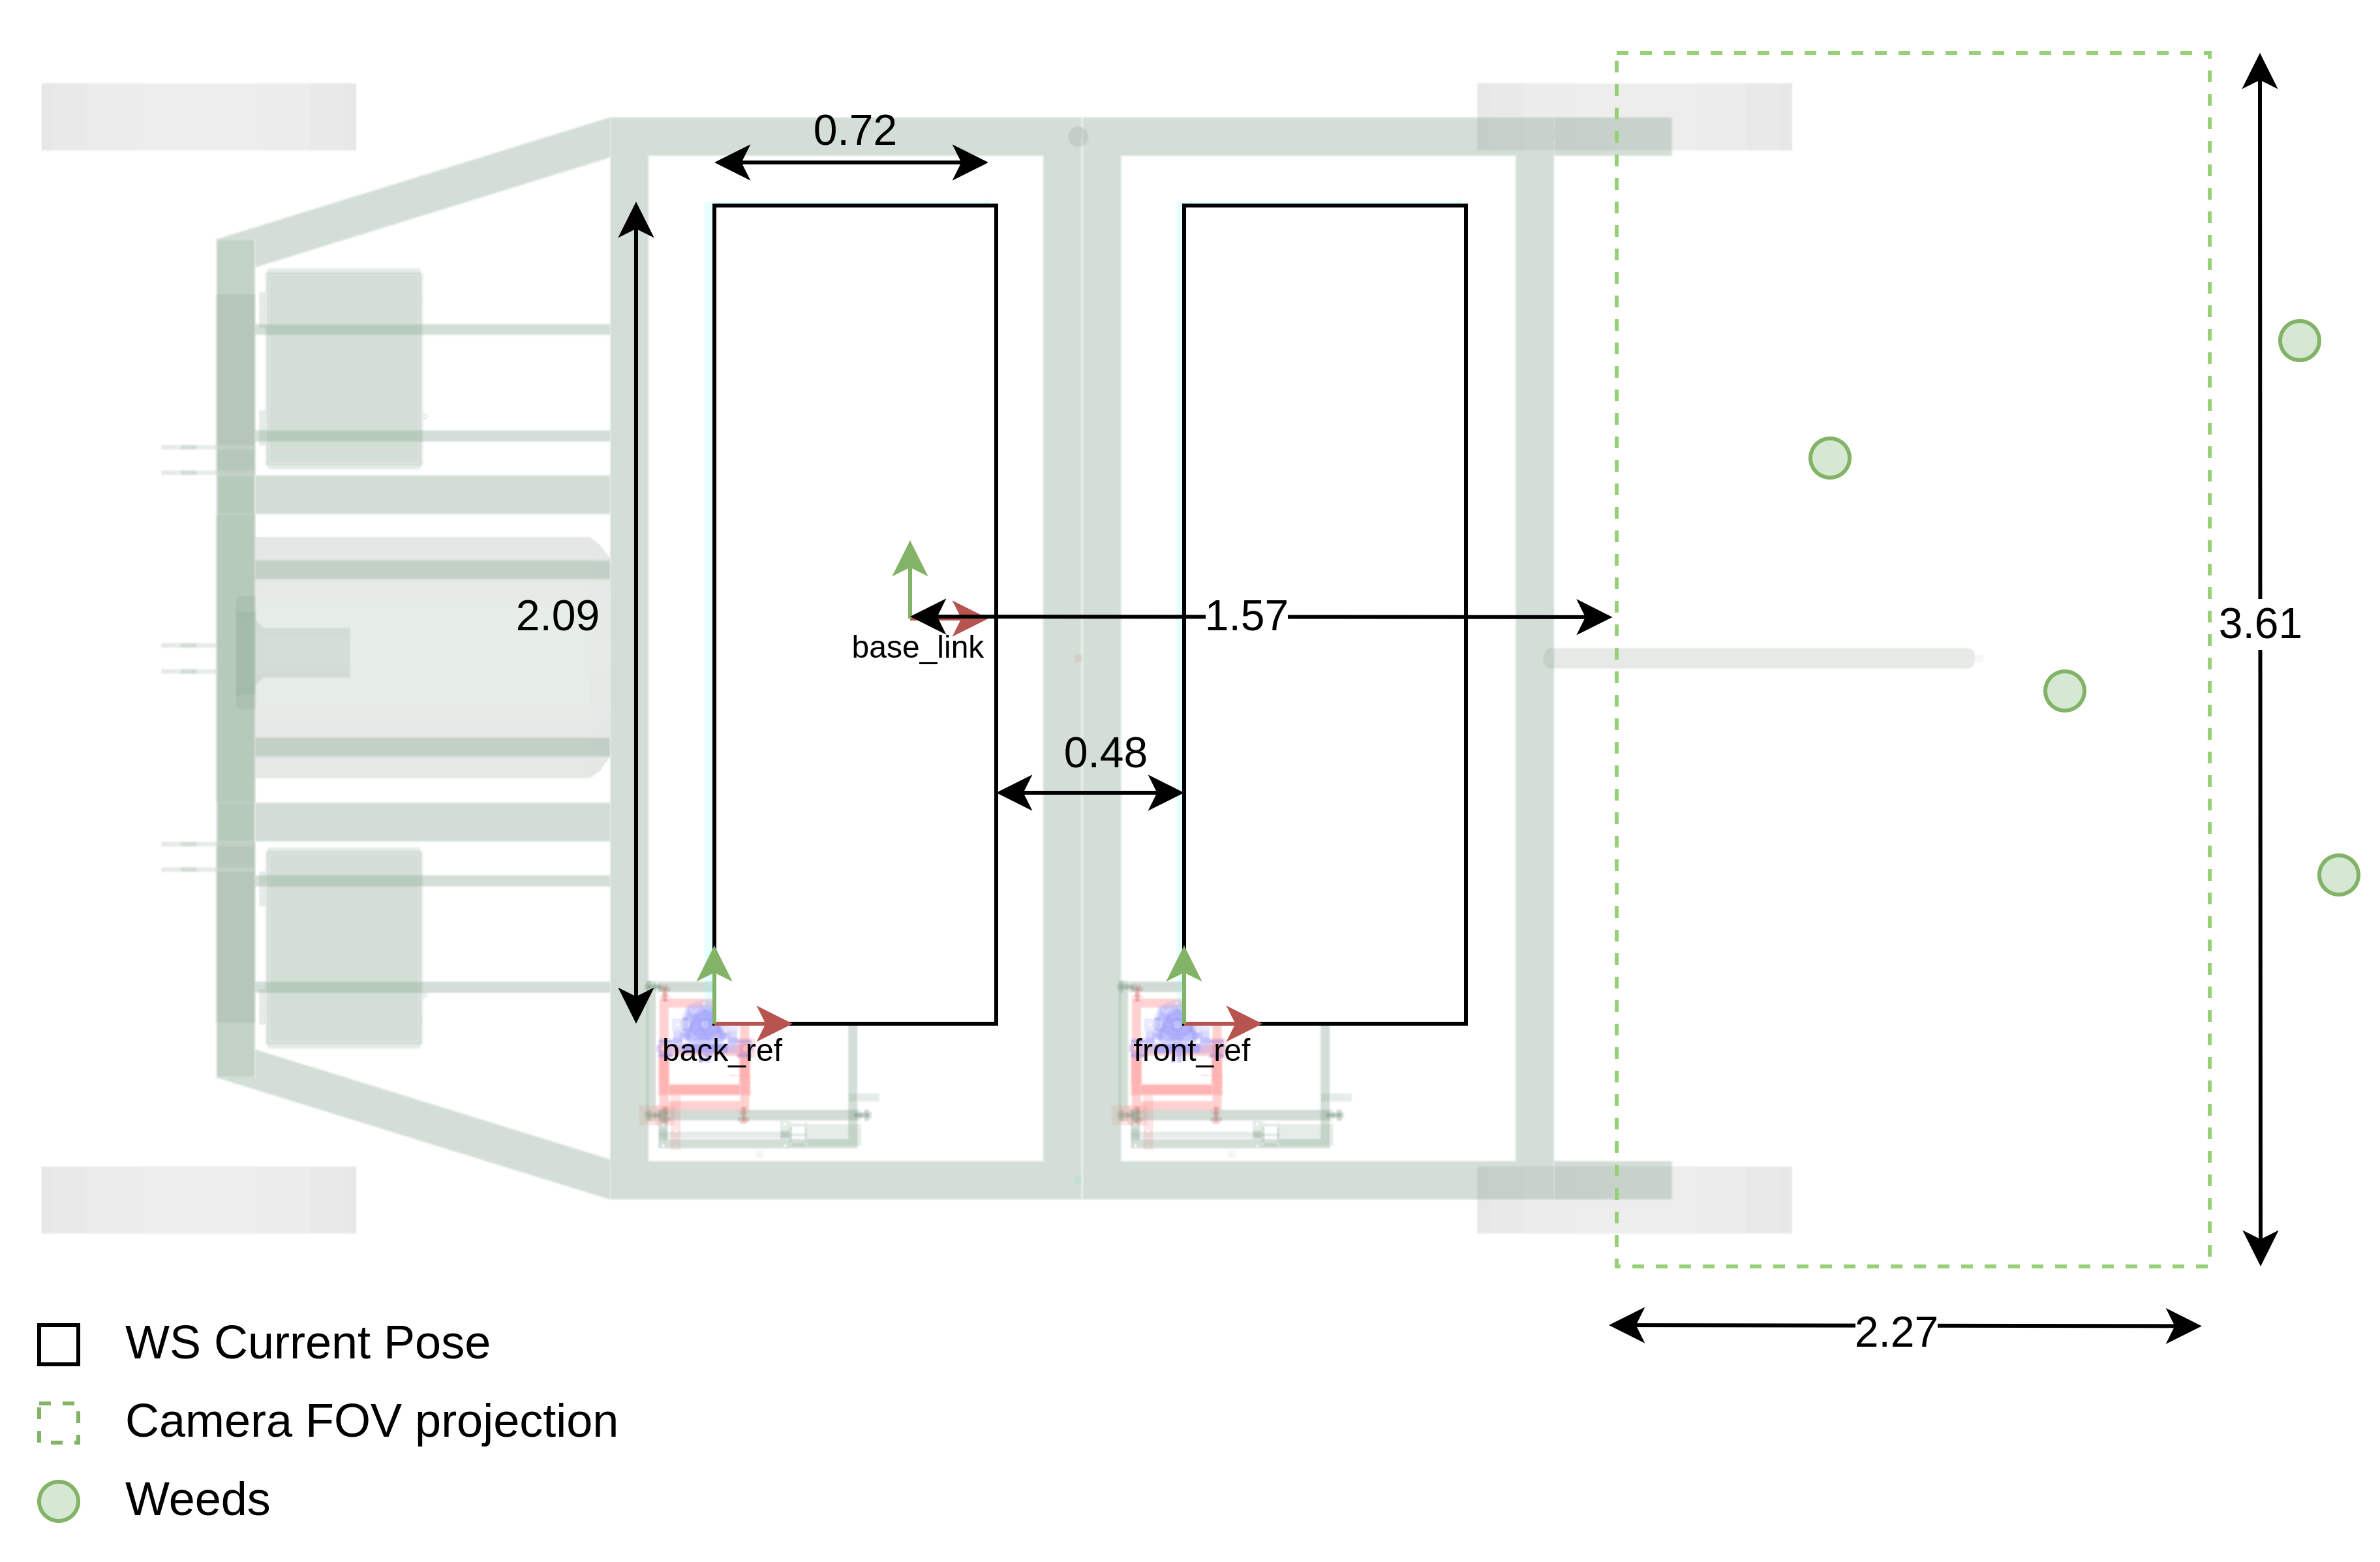
\includegraphics[width=\linewidth]{gfx/ch02/problem_layout.png}
    \caption{Problem Layout Dimentions}
    \label{fig:problem-layout.png}
\end{figure}

\section{Metrics}
Defining a good set of metrics is crucial to establish a good point of comparison between solutions and easily determine the flaws of each method and determine the best solution. Building a dashboard for the summary of each mission was one of the acitivities 

\section{Heuristics}
\lipsum[1]

\section{Graph Search}
\lipsum[1]

\section{Optimization}
\lipsum[1]

%*****************************************
%*****************************************
%*****************************************
%*****************************************
%*****************************************
